\documentclass[12pt]{article}
\usepackage{design_ASC}
\hypersetup{
    colorlinks=true,
    linkcolor=cyan,
    filecolor=magenta,
    urlcolor=blue,}

% Subfigures
\usepackage{subfig}

\setlength\parindent{0pt} %% Do not touch this

%% -----------------------------
%% TITLE
%% -----------------------------
\title{Exercise List \#2} %% Assignment Title

\author{Victor F. Ferrari - RA 187890\\ %% Student name
vferrari@mpc.com.br\\
MO814A/MC937A - Topics in Computer Graphics\\ %% Code and course name
\textsc{Universidade Estadual de Campinas}
}

\date{\today} %% Change "\today" by another date manually
%% -----------------------------
%% -----------------------------

%% %%%%%%%%%%%%%%%%%%%%%%%%%
\begin{document}
\setlength{\droptitle}{-5em}    
%% %%%%%%%%%%%%%%%%%%%%%%%%%
\maketitle

% --------------------------
% Start here
% --------------------------

% %%%%%%%%%%%%%%%%%%%
\section{Color Converter}
% %%%%%%%%%%%%%%%%%%%

The first assigment of the list was to implement a color converter tool, for converting from any supported space to any other. Supports RGB (sRGB), CMY, HSV, XYZ and CIELAB, under Illuminant d50.

\subsection{Details and Usage}
The application was made using \textbf{Python (3)}, in a single file (\texttt{colors.py}). It uses only one external library, \texttt{NumPy}, for operations with arrays. No conversion modules were used. 

The application takes its input values as arguments (\texttt{argv}), and displays the final values in the standard output. The arguments are positional, and can be verified at any time (with details about each parameter) using the \texttt{-h} flag.

Usage: \texttt{python3 colors.py [-h] original final values values values}
\begin{itemize}
        \item \texttt{original}: Name of the original color space. Choices: rgb, cmy, hsv, xyz, cielab. Case sensitive;
        \item \texttt{final}: Name of the desired color space. Choices: rgb, cmy, hsv, xyz, cielab. Case sensitive;
        \item \texttt{values}: Color triplets in the original color space, must be floats. Ranges: RGB $<=$ 255, CMY $<=$ 100.0, HSV Hue $<$ 360.0, HSV Sat/Val $<=$ 1.0. All values except XYZ and CIELAB must be nonnegative. 
\end{itemize}

This program was tested using a Linux-based (Lubuntu) operating system, and verified using \href{http://www.brucelindbloom.com/index.html?ColorCalculator.html}{Bruce Lindbloom's CIE Color Calculator}. Some results were not 100\% equal, but this behavior might happen due to numerical errors in floating point, as some of the conversion methods are implemented as specified in the website as well. For the color spaces not available in the first website, the second source for testing was the \href{http://colorizer.org/}{Colorizer}.

\subsection{Questions}
\subsubsection*{Question 1}
{\bfseries Thinking about color systems, we know that the most used in the computing community is RGB. Explain the reasons for this.}

The RGB model is the most used because it is a simple additive color model, using three values that are directly associated with primary colors (unlike HSV and other color models based on different characteristics of light and color), that can each be represented by a byte integer (0 to 255). That results in a total of $256^3 = 16777216$ possible colors, which is enough for most applications. 

The RGB model also has direct conversions to some other commonly used color spaces (for specific applications). Finally, an additive color space is useful for computer display, since a screen only needs lights for each color per pixel.

\subsubsection*{Question 2}
{\bfseries How is the equivalence given between the RGB and CMY models?}

The CMY and RGB models are complementary. Cyan, magenta and yellow are the result of adding each combination of two of the RGB colors (C: G+B, M: R+B, Y: R+G) while red, green and blue can be acquired subtracting the colors in CMY. So, CMY is a subtractive model while RGB is an additive model, both with the same basis (combining colors to acquire different ones).

Therefore, if both models are in the same scale, the conversion is as simple as inverting the value. So if the scale is from 0 to 1, CMY = 1-RGB and vice-versa.

\subsubsection*{Question 3}
{\bfseries How would you define, in RGB, CMY and HSV:
\begin{itemize}
\item A pure red color
\item A lilac color
\item Yellow
\item Brown
\end{itemize}}

For this answer, RGB values are between 0 and 255 and CMY values are between 0 and 100.0. HSV hue is between 0 and 360 (not inclusive) and HSV saturation and value are between 0 and 1. All floating point answers have at most 2 decimal places.

\begin{itemize}
\item A pure red color
\end{itemize}
RGB: (255, 0, 0); \hspace{1cm} CMY: (0, 100, 100); \hspace{1cm} HSV: (0, 1, 1).\\
Since red is a basic color from RGB, the conversion to CMY is easy. The values for HSV were also very well-behaved.

\begin{itemize}
\item  A lilac color
\end{itemize}
RGB: (200, 162, 200); \hspace{1cm} CMY:(21.57, 36.47, 21.57); \hspace{1cm} HSV:(300, 0.19, 0.78).\\
Lilac is a color that benefits from the CMYK model, because in that one it consists of only magenta and key (black), which is intuitive. When converting to CMY, the magenta is intensified, and some cyan and yellow are necessary for the color, replacing the black.

\begin{itemize}
\item  Yellow
\end{itemize}
CMY: (0, 0, 100); \hspace{1cm} RGB: (255, 255, 0); \hspace{1cm} HSV: (60, 1, 1).\\
Since yellow is a basic color from CMY, the conversion to RGB is easy. The values for HSV were also well-behaved, which shows a pattern in relation to the other two spaces.

\begin{itemize}
\item  Brown
\end{itemize}
RGB: (150, 75, 0); \hspace{1cm} CMY: (41.18, 70.59, 100); \hspace{1cm} HSV: (30, 1, 0.59).\\
Brown is another color that benefits from the CMYK model, because it consists only of magenta (50), yellow (100) and key (black, 41). In the absence of black, more magenta and some cyan are used.

\subsubsection*{Question 4}
{\bfseries What is color?  How is a color characterized?}

Color is how people perceive combinations of certain properties of light. It is a function of the power of the source in various wavelengths, the sensor response to those wavelengths, and the proportion of light reflected off an object's surface for each wavelength.

Since colors are intrinsically related to perception, it only makes sense to define them in the spectrum of visible light. Combining every visible color, the result is white. Most light sources do not produce just one wavelength, but a spectrum, a combination of wavelengths. 

People perceive light through the cone cells, which each type has a different relative response per wavelength. The combination of the spectral radiance of the light and each cone type's response determines how we see color. Electronic sensors use a similar method.

Colors have a lot of different properties that can be use to define each one. It is possible to define a color by a combination of primary colors, such as in the RGB or CMY color spaces, or other properties. These other properties include hue (wavelength), saturation (intensity) and lightness/darkness, used in HSV/HLS color spaces. Other color spaces use both other basic colors and properties to define a color.

\subsubsection*{Question 5}
{\bfseries What is the difference between an additive and a subtractive space?  Explain the application of both (where they are used).}

In an additive space, different colors are produced by superimposing colored lights. In this case, a larger wavelength range is present in the resulting light, so the result of superimposing the colors is \textbf{white}. An example of additive color spaces is the sRGB model. This model is used in many applications, such as computer display.

In a subtractive model, the colors are produced by a sequence of color filters, starting from white, so the result of all filters from this space is \textbf{black}. An example of subtractive color spaces is the CMY model. A similar model, called CMYK (with K being black) is the most used model for printers and similar.

\subsubsection*{Question 6}
{\bfseries What is D50 white point used for?}

The d50 white point is a CIE standard for white, which is used for reference points in definition and conversion of CIE color spaces, such as CIEXYZ and CIELAB. Depending on the reference point used, the final values of color can be different in these models, so the conversion can generate different results in other models.

For the conversions between XYZ and CIELAB, the values of the Illuminant are used directly as a multiplicative or divisive constants. In the conversion between XYZ and RGB, the value is used for chromatic adaptation, generating a different conversion matrix or another step in the conversion.

% %%%%%%%%%%%%%%%%%%%
\section{Scanline Fill Algorithm}
% %%%%%%%%%%%%%%%%%%%

The second assignment of the list was to implement the Scanline Fill algorithm, seen in class, in C++ (14), using the Qt Framework. A graphic application was made that,  given an ordered sequence of vertices, draws a polygon, and can fill it using that algorithm.

\subsection{Details}
This application was made using \textit{Qt Creator}, with \texttt{qmake} and \texttt{make} being used for building. The application does not take any arguments, with every interaction happening during the execution.

The application takes a sequence of clicks, turns into a polygon and draws it. This polygon can be modified (before drawing) by moving the vertices. With the polygon drawn, it can be filled with different colors. Finally, the screen can be cleared, deleting the polygon and allowing the definition of a new one.

\subsection{Usage}
The application has three push buttons, one tool button and a drawing area. 

In the drawing area, vertices can be defined pressing the \textbf{left mouse button}. At the selected points, numbers are drawn, representing the order for the polygon. The polygon can be drawn by pressing the "Draw" button. The color of the drawing can be changed with the "Color" tool.

Only once drawn, the polygon can be filled by pressing the "Fill" button. If a new vertex is created after the polygon is drawn, the application returns to "points mode", showing the numbered vertices. The polygon can be modified using the \textbf{right mouse button}. When it is pressed, the application finds the closest vertex and changes it to that position.

The color can only be changed for the polygon (filled or otherwise), as the numbers representing the points are always blue. The effects of changing the color are immediate. Finally, it is possible to clear the screen by pressing the "Clear" button, resetting the drawing area.

\subsection{Data Structures}
The data structures used for the \textbf{Edge Table (ET)} and for the \textbf{Active Edge Table (AET)} were carefully thought about, and the decision was made based on the complexity of the most used operations.

For the \textbf{ET}, all edges are inserted only once, at the beginning, and every edge is at some point removed. However, the removal happens for the edge with the lowest \texttt{minY} value (if it is equal to the current scan line). Therefore, a sorted array could be used, with amortized $\Op(n)$ complexity for building and $\Op(nlogn)$ complexity for sorting, and removals are done in constant time. However, a \textbf{priority queue} was chosen for the ET, in the form of a \textbf{minimum heap}. The complexity is not much better, with $\Op(n)$ complexity for building and $\Op(logn)$ complexity for removal of each element, but it's easier to work with in C++ (a \textbf{vector} was used as container).

For the \textbf{AET}, there is no order for insertion and removal in each iteration, so the removal of an arbitrary element ought to be done in constant time, if possible, as well as the insertion at the end or beginning. Yet, no searches are necessary if sorting is possible, so every access goes through the entire structure. For those reasons, a \textbf{list} was chosen for the AET, specifically a \textbf{forward list}, or singly-linked list. Insertion of an element at the beginning can be done in constant time, as well as the removal of an arbitrary element, once it is located. Locating the element is not a problem, because every element has to be tested anyway. Sorting can have $\Op(nlogn)$ complexity.

\subsection{Results}
This application was tested using a Linux-based (Lubuntu) operating system, and was successful in its objective. It was possible to create polygons in which the filling algorithm didn't work as expected, but for most well-behaved (even with multiple auto-intersections) polygons, it worked without a problem.

\begin{figure}
    \centering
    \subfloat[Convex - Without Auto-intersections]{
    \label{fig:poly1}
    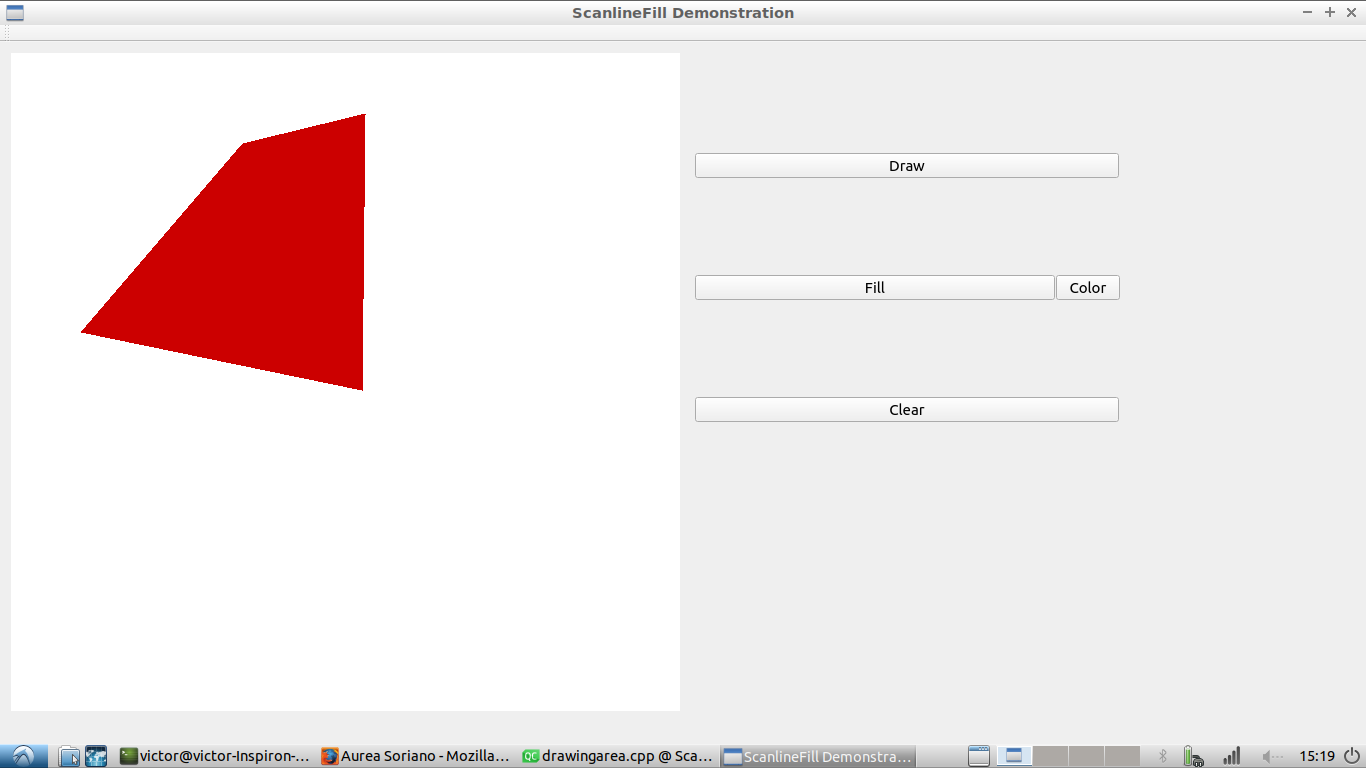
\includegraphics[width=0.5\textwidth]{./images/common.png}
    }
    \subfloat[Concave - Without Auto-intersections]{
    \label{fig:poly2}
    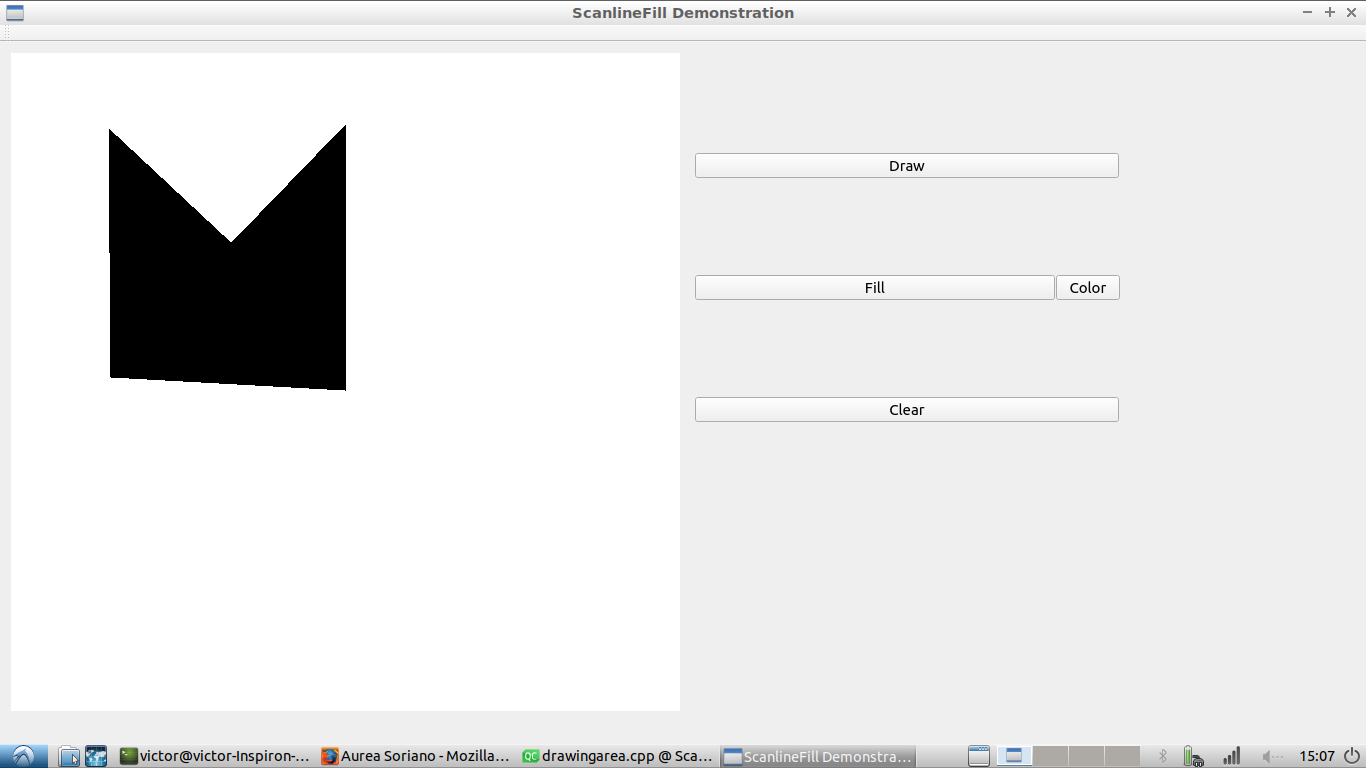
\includegraphics[width=0.5\textwidth]{./images/concave.png}
    }
    \qquad
    \subfloat[With Auto-intersections]{
    \label{fig:poly3}
    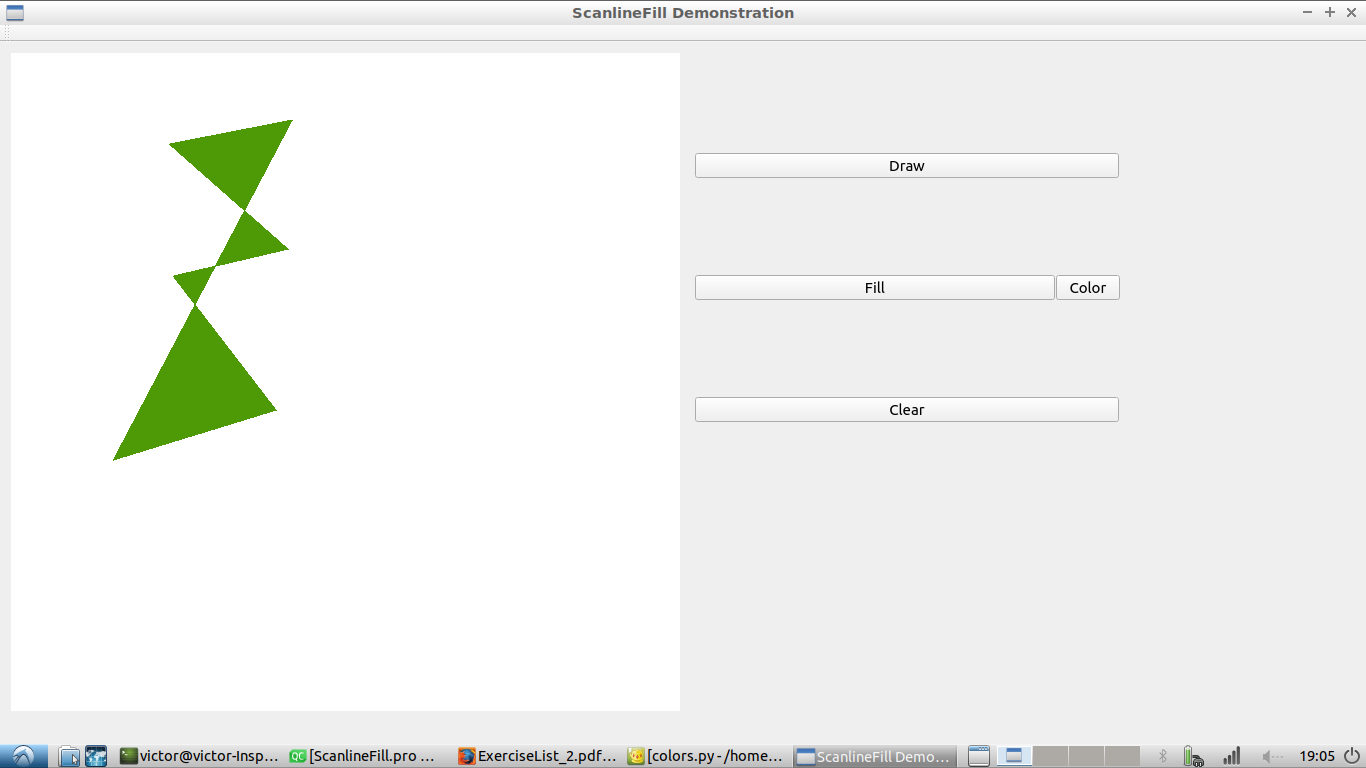
\includegraphics[width=0.8\textwidth]{./images/auto_int.png}
    }
    \caption{Polygons filled using the Scanline Fill Algorithm in Qt.}
    \label{fig:poly}
\end{figure}

The result for polygons without auto-intersections can be found in Figures \ref{fig:poly1} and \ref{fig:poly2} (convex and concave, respectively), and the result for a polygon with auto-intersections can be found in Figure \ref{fig:poly3}.
\end{document}